\section{Tích hợp Business Intelligence và Xây dựng Dashboard}

Sau khi hoàn tất quá trình ETL và khai phá dữ liệu, nhóm thực hiện xây dựng lớp trình bày (Presentation Layer) sử dụng song song hai nền tảng: \textbf{Microsoft Power BI Desktop} (cho đối tượng quản trị / lãnh đạo) và \textbf{Streamlit} (cho phân tích viên kỹ thuật). Mục tiêu là chuyển đổi kết quả phân tích từ SQL và Python thành hệ thống báo cáo tương tác phục vụ ra quyết định \cite{kimball2013}.

\subsection{Hiện thực hóa mô hình dữ liệu trong Power BI}

Dữ liệu từ Gold Layer trong PostgreSQL được nạp vào Power BI thông qua hai phương án:
\begin{itemize}
    \item \textbf{DirectQuery / Import qua Npgsql ODBC} -- chế độ production khi PostgreSQL đã được triển khai.
    \item \textbf{CSV Import} qua script \texttt{tools/export\_gold\_for\_powerbi.py} -- chế độ thử nghiệm nhanh, không cần PostgreSQL. Script này xuất 4 tệp CSV (\texttt{fact\_market\_daily.csv}, \texttt{dim\_coin.csv}, \texttt{dim\_date.csv}, \texttt{dim\_category.csv}) tương ứng các bảng trong Star Schema.
\end{itemize}

Trong Model View của Power BI, kiến trúc Star Schema được hiện thực hóa với bảng sự kiện trung tâm \texttt{fact\_market\_daily} kết nối với ba bảng chiều qua quan hệ \emph{many-to-one} (Hình \ref{fig:pbi_model}).

\begin{figure}[H]
    \centering
    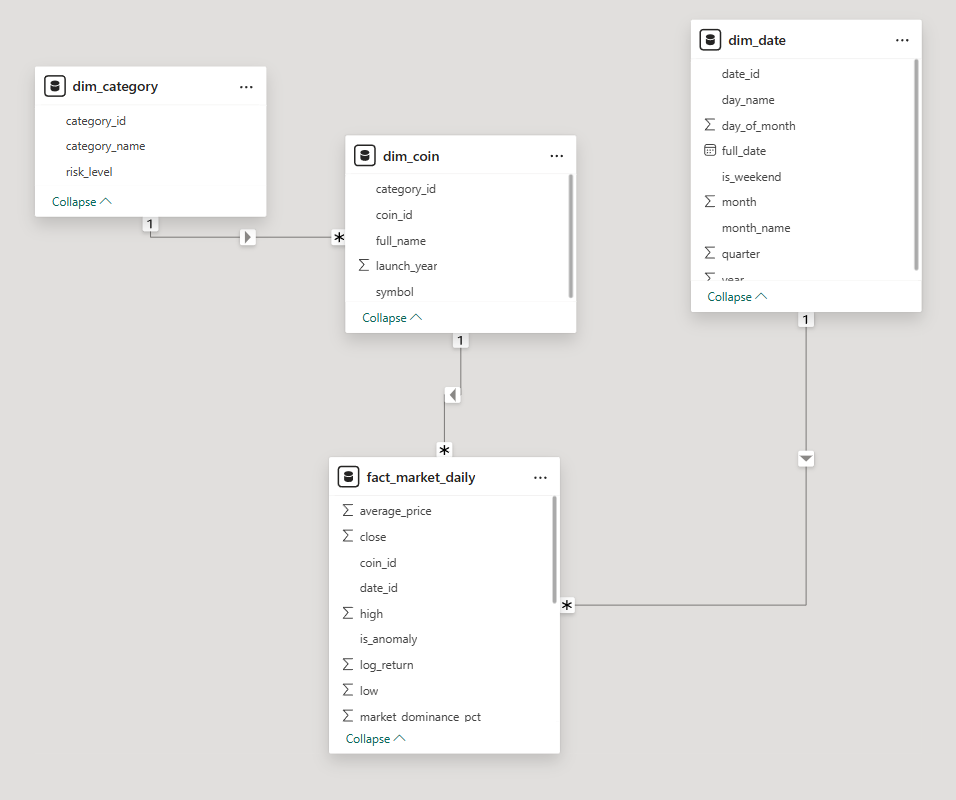
\includegraphics[width=0.95\textwidth]{Images/PBI/pbi_model_view.png}
    \caption{Power BI Model View -- Star Schema với 3 active relationships}
    \label{fig:pbi_model}
\end{figure}

Việc đánh dấu \texttt{dim\_date} bằng \emph{Mark as date table} cho phép Power BI tự động sinh \texttt{Date Hierarchy} (Year $\to$ Quarter $\to$ Month $\to$ Day), phục vụ cho thao tác Drill-down -- một tính năng nền tảng của OLAP \cite{chaudhuri1997}.

\subsection{Phân hệ 1 -- Crypto Market Overview}

Phân hệ này phục vụ nhu cầu theo dõi tổng quan thị trường, dành cho lãnh đạo và nhà đầu tư cá nhân.

\begin{figure}[H]
    \centering
    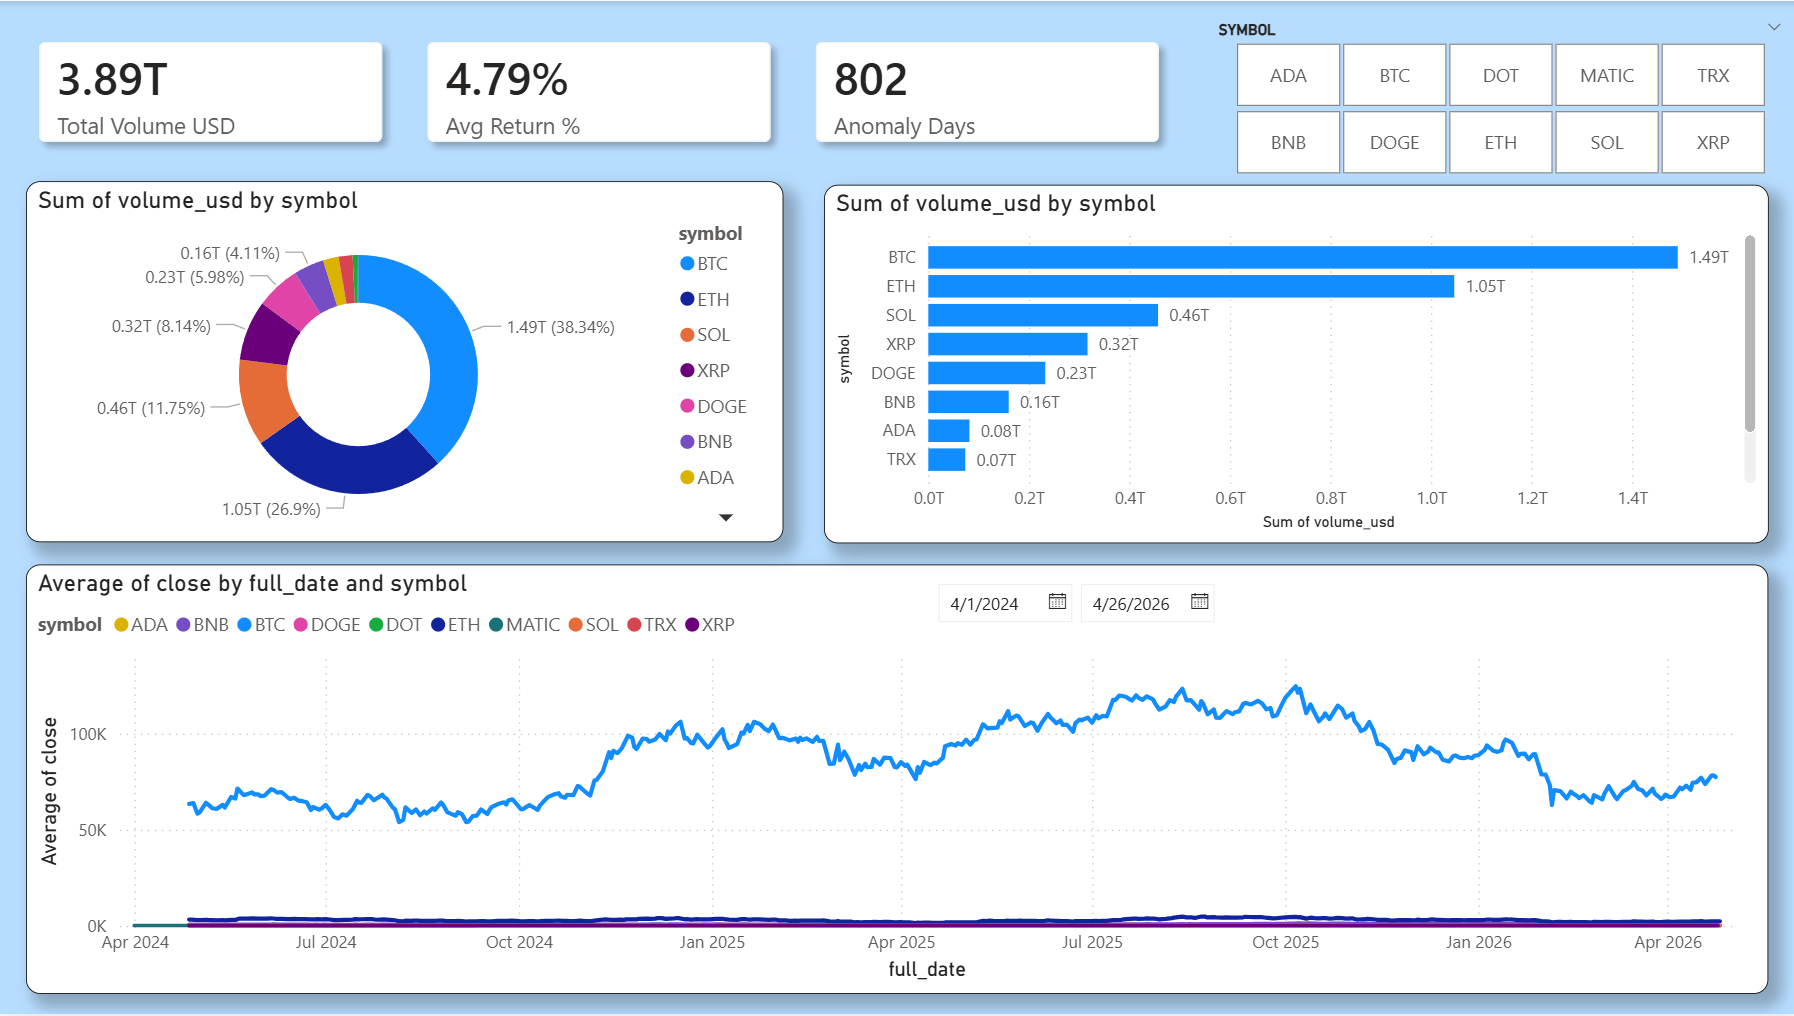
\includegraphics[width=\textwidth]{Images/PBI/dashboard_overview.png}
    \caption{Power BI Dashboard -- Crypto Market Overview}
    \label{fig:pbi_overview}
\end{figure}

Dashboard này (Hình \ref{fig:pbi_overview}) gồm bốn vùng visual chính:
\begin{itemize}
    \item \textbf{KPI Cards (hàng đầu):} 5 số liệu tổng quan -- Total Volume USD ($\sim\$3{,}933$B), Avg Daily Return ($+0.053\%$), Anomaly Days (874 phiên, $\sim 12\%$), Bull/Bear Days, và Coins Selected. Dùng DAX measure như:
    \begin{verbatim}
    Total Volume USD = SUM(fact_market_daily[volume_usd])
    Anomaly Days = CALCULATE(COUNTROWS(fact_market_daily),
                             fact_market_daily[is_anomaly] = TRUE())
    \end{verbatim}
    \item \textbf{Daily Close Price (line chart):} Top-5 coin theo volume, chuẩn hoá về 1.0 đầu kỳ -- cho phép so sánh hiệu suất tích lũy trực quan.
    \item \textbf{Market Dominance (donut):} Tỷ trọng \texttt{volume\_usd} của từng coin -- BTC chiếm $\sim 25\%$, ETH $\sim 20\%$, phần còn lại chia đều.
    \item \textbf{Volume Leaderboard (horizontal bar):} Xếp hạng thanh khoản trung bình ngày -- giúp xác định coin nào có liquidity đủ cho giao dịch khối lượng lớn.
\end{itemize}

\subsection{Phân hệ 2 -- Data Mining Insights}

Phân hệ này trực quan hoá kết quả của các kỹ thuật khai phá dữ liệu (mục 4.3), phục vụ phòng phân tích định lượng.

\begin{figure}[H]
    \centering
    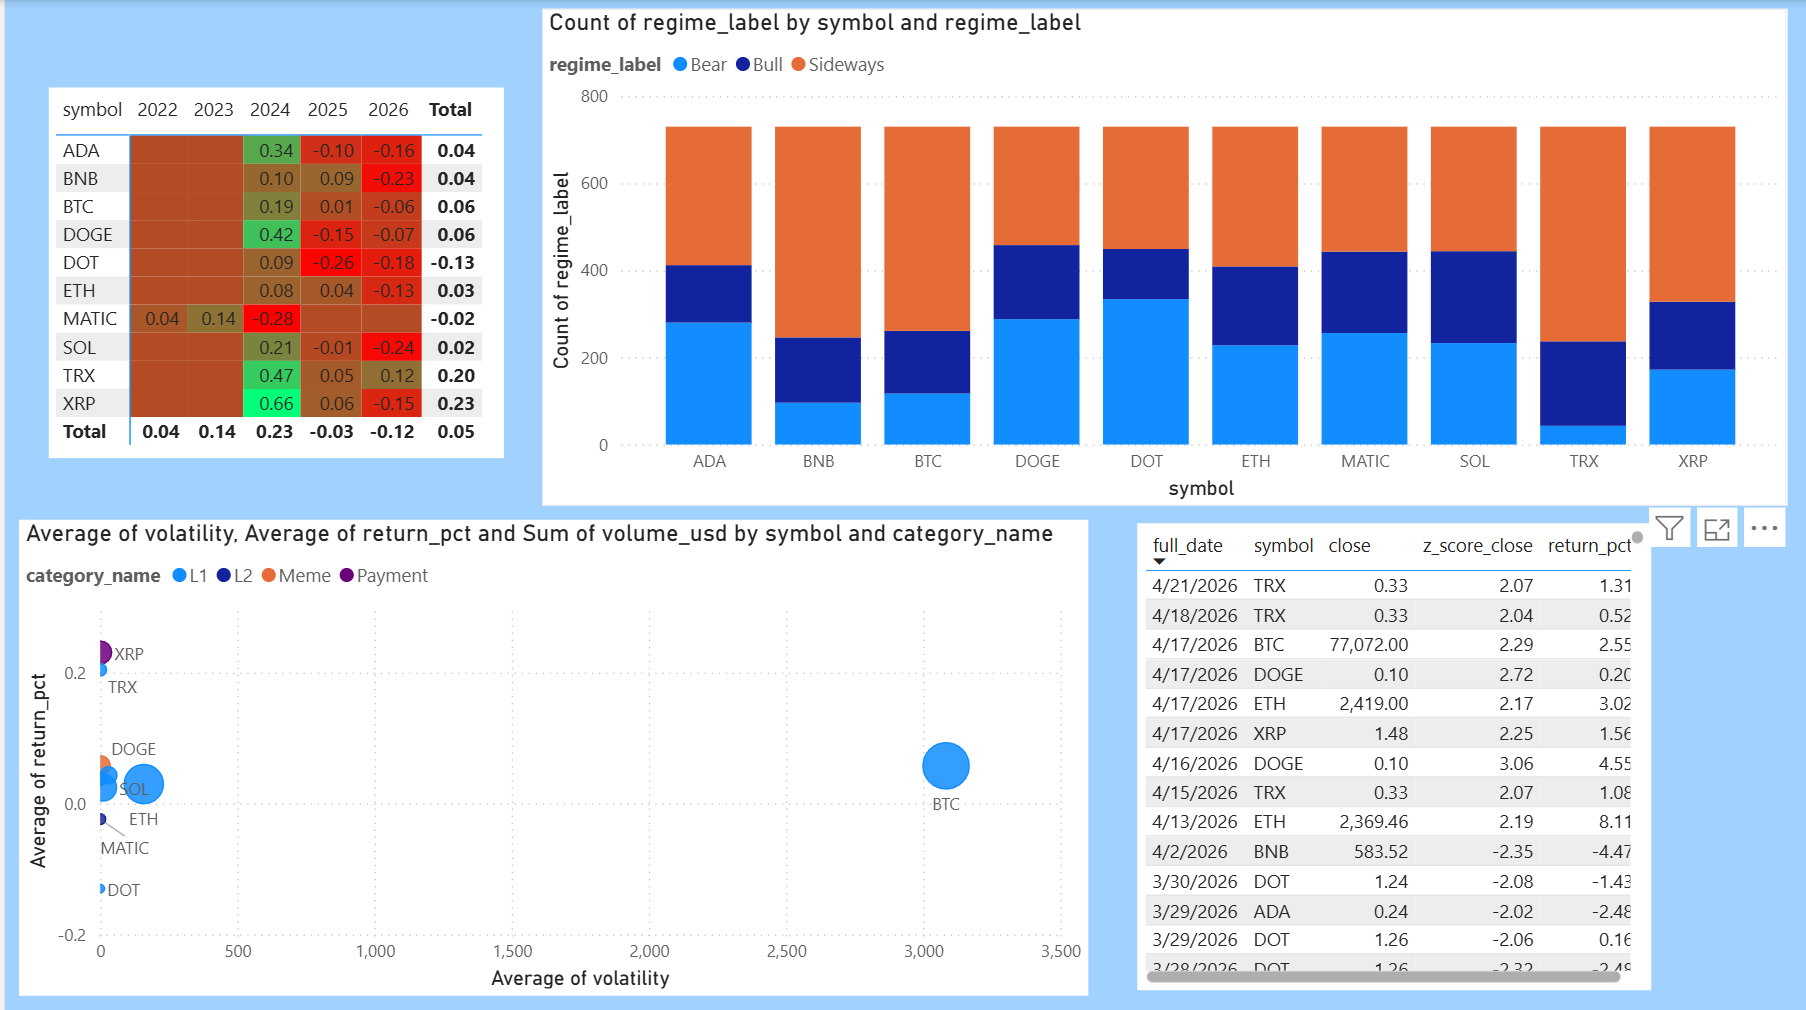
\includegraphics[width=\textwidth]{Images/PBI/dashboard_mining.png}
    \caption{Power BI Dashboard -- Data Mining Insights}
    \label{fig:pbi_mining}
\end{figure}

Dashboard này (Hình \ref{fig:pbi_mining}) gồm bốn visual:
\begin{itemize}
    \item \textbf{Risk-Return Scatter (scatter plot):} Trục X = Volatility (std return), trục Y = Mean Return, kích thước bubble = Volume, màu = Category. Visual này tái hiện kết quả K-Means clustering ở mục 4.3.2 trong môi trường tương tác -- người dùng có thể click vào một bubble để filter các visual khác.
    \item \textbf{Regime Distribution (stacked bar):} Tỷ lệ ngày Bull/Sideways/Bear cho từng coin. Màu xanh lá $=$ Bull, vàng $=$ Sideways, đỏ $=$ Bear.
    \item \textbf{Top Anomalies per Coin (horizontal bar):} Số phiên có $|z\_score| > 2$ -- cho thấy TRX là coin có nhiều anomaly nhất (107 phiên).
    \item \textbf{Top-10 Extreme Anomalies (table):} Danh sách phiên cực đoan nhất theo $|z|$ -- tham chiếu trực tiếp \texttt{gold.v\_top\_anomalies} view.
\end{itemize}

\subsection{Tính năng OLAP Drill-down}

Đặc trưng quan trọng của Power BI là khả năng \textbf{drill-down} dọc theo Date Hierarchy của \texttt{dim\_date} \cite{chaudhuri1997}. Hình \ref{fig:pbi_drill} minh hoạ thao tác drill-down 3 cấp cho BTC: từ tổng hợp năm $\to$ quý $\to$ tháng.

\begin{figure}[H]
    \centering
    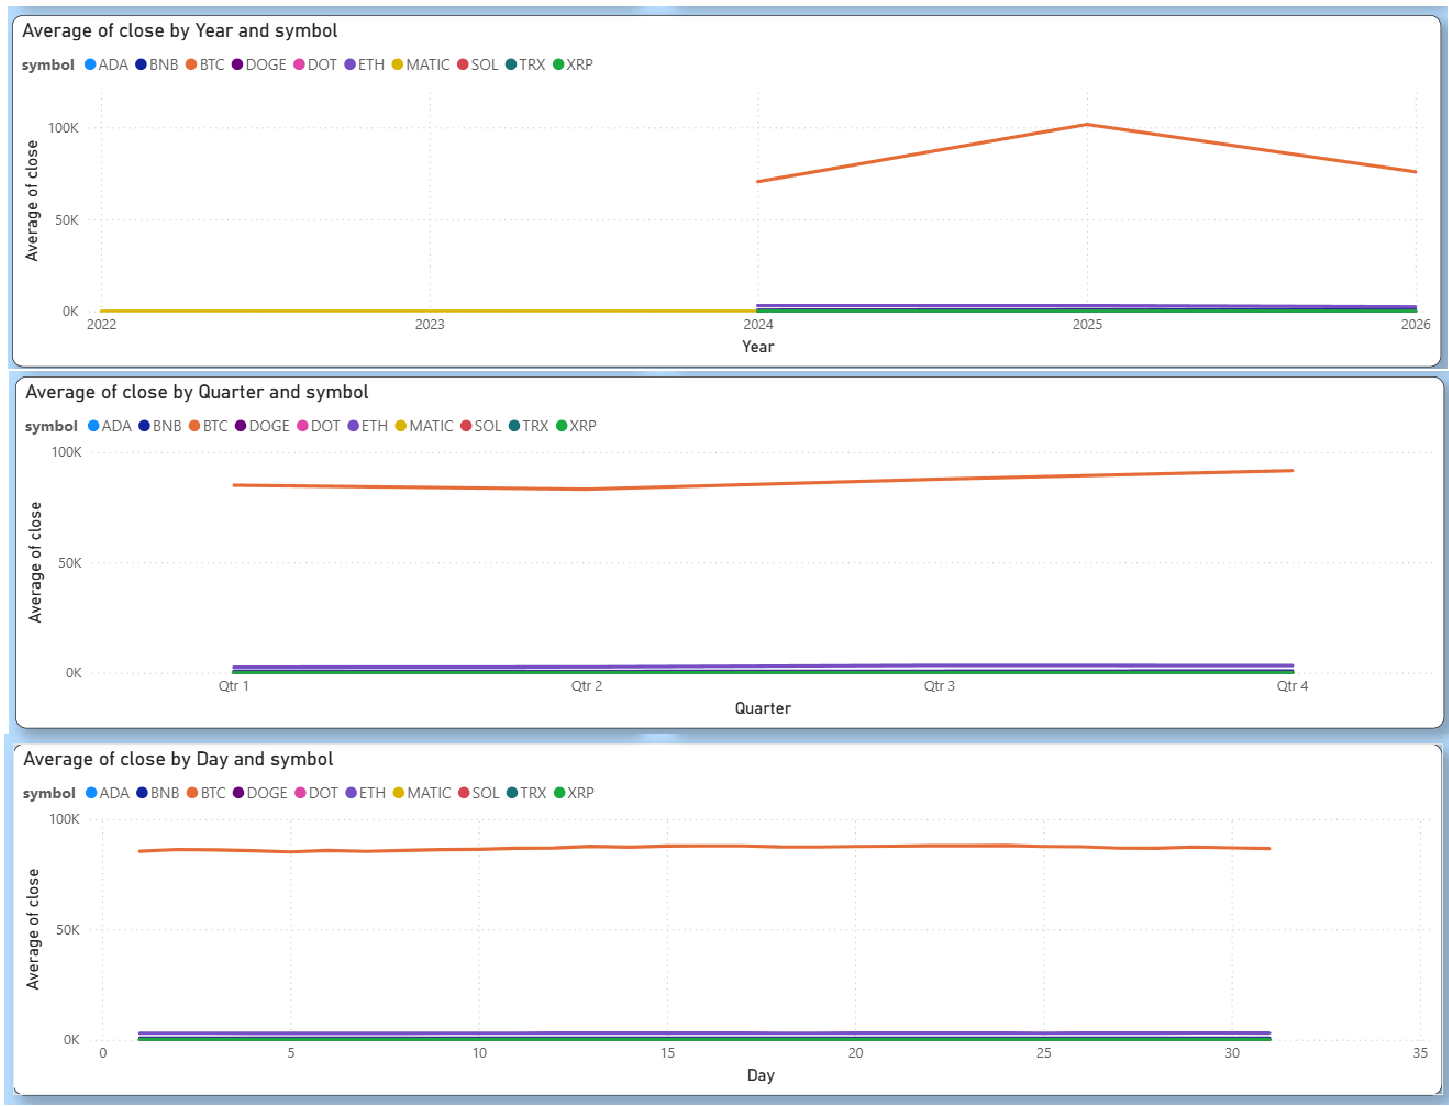
\includegraphics[width=\textwidth]{Images/PBI/pbi_drilldown.png}
    \caption{OLAP Drill-down: Year $\to$ Quarter $\to$ Month cho BTC}
    \label{fig:pbi_drill}
\end{figure}

Quy trình thao tác:
\begin{enumerate}
    \item \textbf{Level 1 (Year):} Bar chart hiển thị tổng \texttt{return\_pct} mỗi năm.
    \item \textbf{Level 2 (Quarter):} Click chuột phải $\to$ Drill down vào năm có biến động lớn nhất -- bar chart đổi sang Q1/Q2/Q3/Q4.
    \item \textbf{Level 3 (Month):} Tiếp tục drill down vào quý có anomaly cao nhất -- bar chart đổi sang từng tháng, lộ ra tháng cụ thể có sự kiện.
\end{enumerate}

Đây chính là chuỗi thao tác OLAP cốt lõi (Drill-down + Roll-up) mà Kimball mô tả là \emph{``the killer feature of dimensional modeling''} \cite{kimball2013}.

\subsection{Ứng dụng Streamlit Dashboard}

Bên cạnh Power BI, nhóm còn xây dựng một dashboard tương tác bằng Python Streamlit (\texttt{streamlit\_crypto.py}). Ứng dụng kết nối trực tiếp PostgreSQL hoặc CSV (qua wrapper \texttt{streamlit\_crypto\_csv.py}), cho phép người dùng tùy chỉnh tham số và quan sát các biểu đồ Plotly trên nền tảng Web -- chi tiết xem chương Demo (mục 6).

\subsection{So sánh hai nền tảng}

\begin{table}[H]
\centering
\caption{So sánh Power BI và Streamlit cho dự án CryptoDW}
\label{tab:pbi_vs_streamlit}
\small
\begin{tabular}{@{}lll@{}}
\toprule
\textbf{Khía cạnh} & \textbf{Power BI Desktop} & \textbf{Streamlit} \\ \midrule
Đối tượng người dùng & Lãnh đạo, không-coder & Phân tích viên kỹ thuật \\
Học cách dùng & Drag \& drop, dễ & Cần biết Python \\
Tuỳ biến chuyên sâu & Hạn chế (DAX) & Toàn quyền (Python + Plotly) \\
Triển khai chia sẻ & Power BI Service (cloud) & Streamlit Cloud / Docker \\
Chi phí licence & Cần PRO licence cho share & Miễn phí mã nguồn mở \\
Refresh dữ liệu & Manual / Scheduled & Realtime khi có request \\ \bottomrule
\end{tabular}
\end{table}

Việc cung cấp song song cả hai nền tảng đáp ứng được nhu cầu đa tầng trong tổ chức: lãnh đạo dùng Power BI để xem báo cáo tổng hợp định kỳ, trong khi phân tích viên dùng Streamlit để khai thác dữ liệu chuyên sâu \cite{vanderplas2016}.
